%-----------------------------------LICENSE------------------------------------%
%   This file is part of tikz_figures.                                         %
%                                                                              %
%   tikz_figures is free software: you can redistribute it and/or              %
%   modify it it under the terms of the GNU General Public License as          %
%   published by the Free Software Foundation, either version 3 of the         %
%   License, or (at your option) any later version.                            %
%                                                                              %
%   tikz_figures is distributed in the hope that it will be useful,            %
%   but WITHOUT ANY WARRANTY; without even the implied warranty of             %
%   MERCHANTABILITY or FITNESS FOR A PARTICULAR PURPOSE.  See the              %
%   GNU General Public License for more details.                               %
%                                                                              %
%   You should have received a copy of the GNU General Public License along    %
%   with tikz_figures.  If not, see <https://www.gnu.org/licenses/>.           %
%------------------------------------------------------------------------------%

% Use the standalone class for displaying the tikz image on a small PDF.
\documentclass[crop, tikz]{standalone}

% Import the tikz package to use for the drawing.
\usepackage{tikz}

% Tikz packages used.
\usetikzlibrary{arrows, shapes, positioning}

% Begin the document.
\begin{document}

    % Draw the figure.
    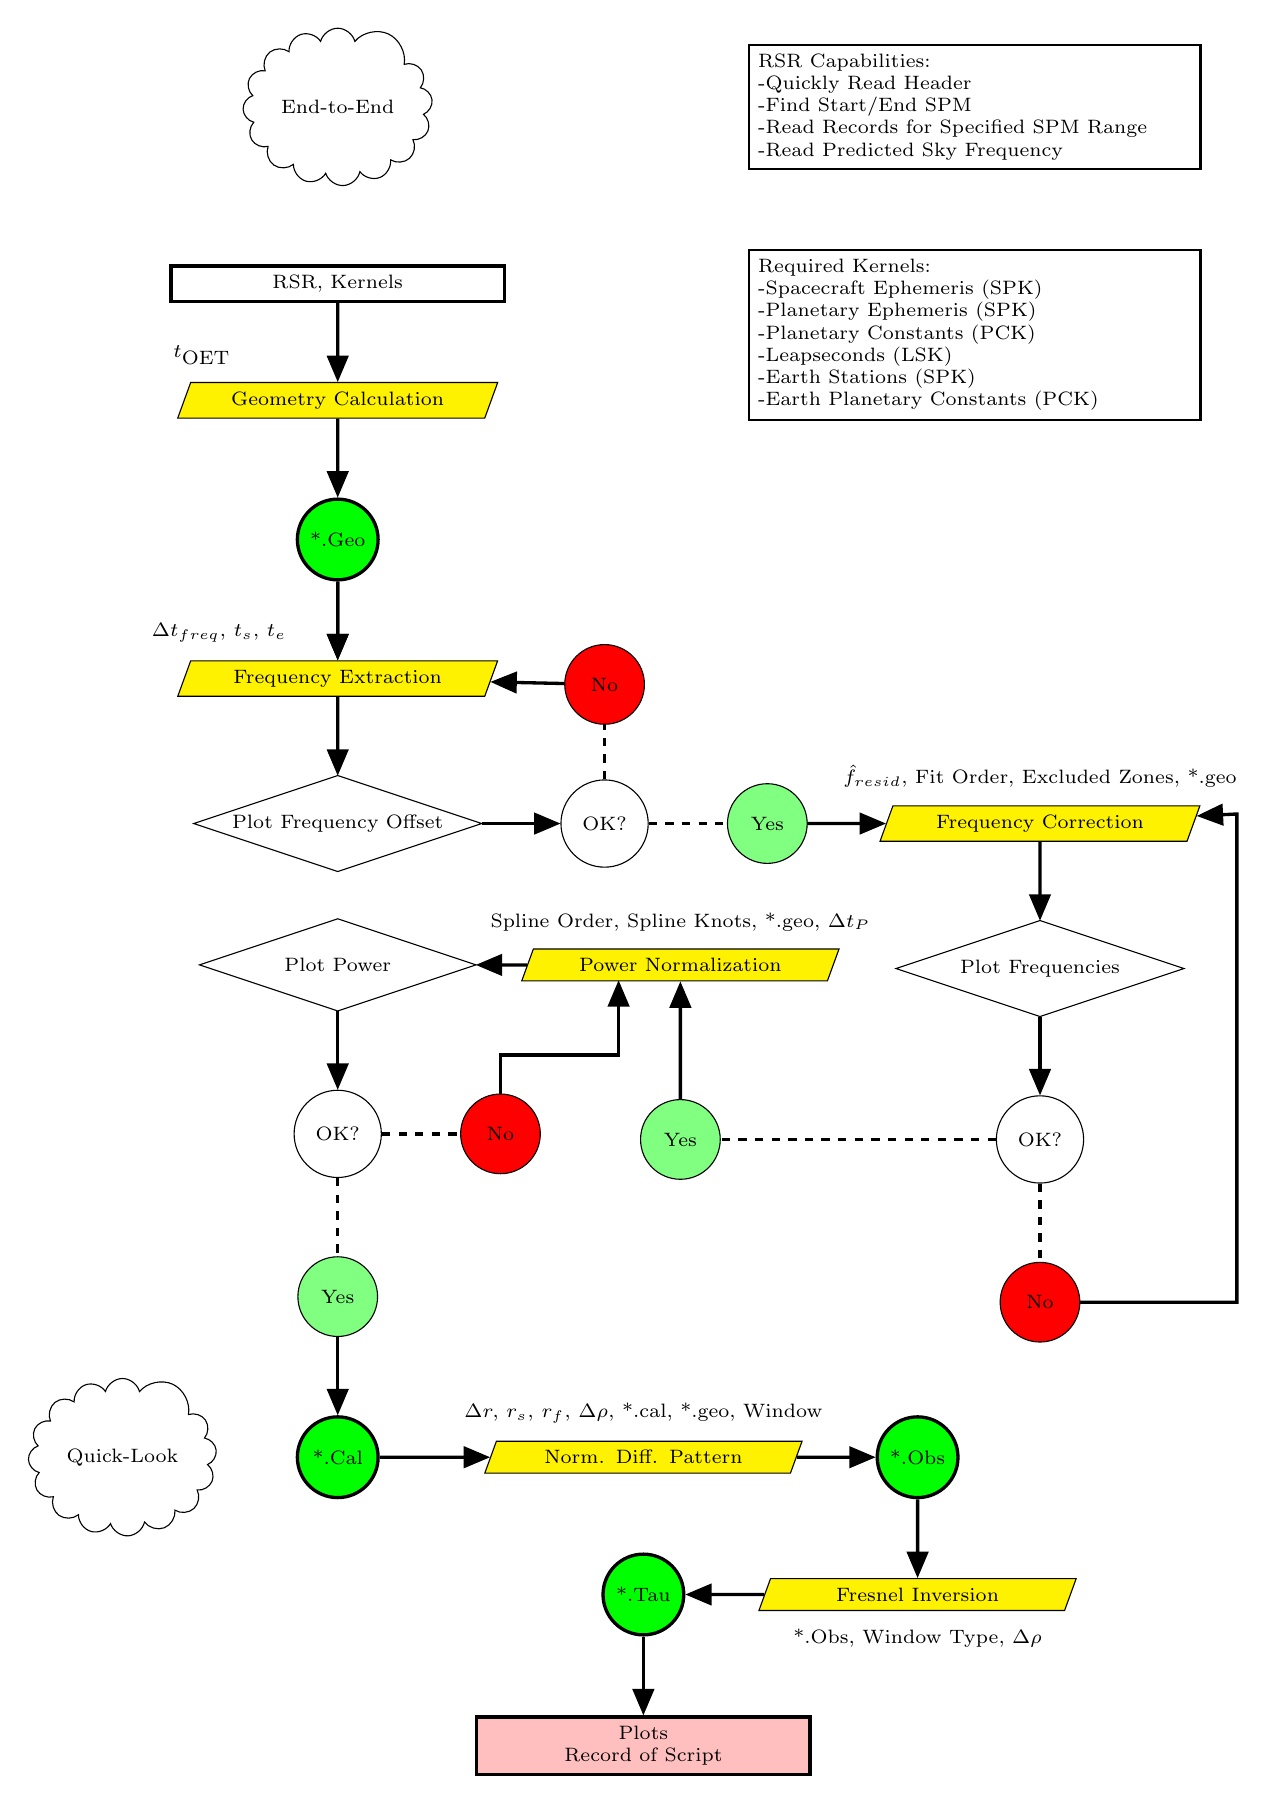
\begin{tikzpicture}[%
        font = \scriptsize,
        > = {triangle 45},
        roundnode/.style = {%
            circle,
            draw = black,
            very thick,
            text width = 2em,
            text centered,
            fill = green
        },
        squarenode/.style = {%
            rectangle,
            text width = 4em,
            text centered,
            draw = black,
            very thick,
            fill = blue!50!white
        },
        bignode/.style = {%
            rectangle,
            draw = black,
            very thick,
            text width = 4cm,
            text centered
        },
        bigbig/.style = {%
            rectangle,
            draw = black,
            thick,
            text width = 5.5cm
        },
        every edge/.style = {%
            draw = black,
            very thick
        },
        trapanode/.style = {%
            trapezium,
            trapezium left angle = 70,
            trapezium right angle = -70,
            draw = black,
            fill = yellow,
            text width = 3.5cm,
            text centered
        },
        dianode/.style = {%
            diamond,
            draw = black,
            text width = 3cm,
            text centered,
            aspect = 3,
            inner sep = 0,
            outer sep = 0
        },
        qnode/.style = {%
            circle,
            draw = black,
            text width = 8mm,
            text centered
        },
        nonode/.style = {%
            circle,
            draw = black,
            fill = red,
            text width = 1cm,
            text centered,
            inner sep=0,
            outer sep=0
        },
        yenode/.style = {%
            circle,
            draw = black,
            fill = green!50!white,
            text width = 1cm,
            text centered,
            inner sep = 0,
            outer sep = 0
        }
    ]
        \node[%
            cloud,
            cloud puffs = 15.7,
            cloud ignores aspect,
            minimum height = 2cm,
            align = center,
            draw,
            aspect = 3
        ] (0) {End-to-End};
        \node[bignode] (1) [below = of 0] {RSR, Kernels};
        \node[trapanode] (2) [below = of 1] {Geometry Calculation};
        \node[above left=1mm and 10mm of 2] {$t_{\textrm{OET}}$};
        \node[roundnode] (3) [below = of 2] {*.Geo};
        \node[trapanode] (4) [below = of 3] {Frequency Extraction};
        \node[above left = 1mm and 3mm of 4] {%
            $\Delta{t}_{freq},\,t_{s},\,t_{e}$
        };
        \node[dianode] (5)  [below = of 4] {Plot Frequency Offset};
        \node[qnode] (6)  [right = of 5] {OK?};
        \node[nonode] (6n) [above = 7mm of 6] {No};
        \node[yenode] (6y) [right = of 6] {Yes};
        \node[trapanode] (7) [right = of 6y] {Frequency Correction};
        \node[dianode] (7a) [below = of 7] {Plot Frequencies};
        \node[qnode] (8) [below = of 7a] {OK?};
        \node[nonode] (8n) [below = of 8] {No};
        \node[yenode] (8y) [left = 3.5cm of 8] {Yes};
        \node[trapanode] (9) [above = 1.5cm of 8y] {Power Normalization};
        \node[above = 1mm of 7] {%
            $\hat{f}_{resid}$, Fit Order, Excluded Zones, *.geo
        };
        \node[above=1mm of 9] {%
            Spline Order, Spline Knots, *.geo, $\Delta{t}_{P}$
        };
        \node[dianode] (10) [below = 6mm of 5] {Plot Power};
        \node[qnode] (11)  [below = of 10] {OK?};
        \node[nonode] (11n) [right = 1cm of 11] {No};
        \node[yenode] (11y) [below = 1cm of 11] {Yes};
        \node[roundnode] (12) [below = of 11y] {*.Cal};
        \node[trapanode] (13) [right = 1.4cm of 12] {Norm. Diff. Pattern};
        \node[above=1mm of 13] {%
            $\Delta{r},\,r_{s},\,r_{f},\,\Delta\rho,$ *.cal, *.geo, Window
        };
        \node[roundnode] (14)  [right=1cm of 13]  {\scriptsize{*.Obs}};
        \node[trapanode] (15)  [below=of 14] {\scriptsize{Fresnel Inversion}};
        \node[roundnode] (16)  [left =of 15] {\scriptsize{*.Tau}};
        \node[bignode, fill = pink] (END) [below = of 16] {%
            Plots\\
            Record of Script
        };
        \node[below = 1mm of 15] {*.Obs, Window Type, $\Delta\rho$};
        \node[%
            cloud,
            cloud puffs = 15.7,
            cloud ignores aspect,
            minimum height = 2cm,
            align = center,
            draw
        ] (QL) [left = of 12] {Quick-Look};

        \node[bigbig] (RSR) [right = 4 cm of 0] {%
            RSR Capabilities:\\
            -Quickly Read Header\\
            -Find Start/End SPM\\
            -Read Records for Specified SPM Range\\
            -Read Predicted Sky Frequency
        };

        \node[bigbig] (Ker) [below = of RSR] {%
            Required Kernels:\\
            -Spacecraft Ephemeris (SPK)\\
            -Planetary Ephemeris (SPK)\\
            -Planetary Constants (PCK)\\
            -Leapseconds (LSK)\\
            -Earth Stations (SPK)\\
            -Earth Planetary Constants (PCK)
        };

        %Lines.
        \path[->] (1) edge (2);
        \path[->] (2) edge (3);
        \path[->] (3) edge (4);
        \path[->] (3) edge (4);
        \path[->] (4) edge (5);
        \path[->] (5) edge (6);
        \path[-, dashed] (6) edge (6n);
        \path[->] (6n) edge (4);
        \path[-, dashed] (6) edge (6y);
        \path[->] (6y) edge (7);
        \path[->] (7) edge (7a);
        \path[->] (7a) edge (8);
        \path[-, dashed] (8) edge (8n);
        \path[-, dashed] (8) edge (8y);
        \path[->] (8y) edge (9);
        \path[->] (9) edge (10);
        \path[->] (10) edge (11);
        \path[-, dashed] (11) edge (11n);
        \path[-, dashed] (11) edge (11y);
        \path[->] (11y) edge (12);
        \path[->] (12) edge (13);
        \path[->] (13) edge (14);
        \path[->] (14) edge (15);
        \path[->] (15) edge (16);
        \path[->] (16) edge (END);

        \begin{scope}[%
            ->,
            draw = black,
            very thick
        ]
            \draw (8n) to ++(2.5cm, 0.0) to ++(0.0, 6.2cm) to (7);
            \draw (11n) to ++(0.0, 1.0cm) to ++(1.5cm, 0.0) to ++(0.0, 0.95cm);
        \end{scope}
    \end{tikzpicture}
\end{document}
